\documentclass[a4paper,10pt]{article}
\usepackage[left=2cm, right=2cm, top=2cm, bottom=2cm]{geometry}
\usepackage{titlesec, enumitem, hyperref, graphicx}
\usepackage{xcolor}
\usepackage{fontawesome5}
\usepackage{tabularx}
\usepackage{ltablex}
\usepackage{tikz}

% Tikz Libraries
\usetikzlibrary{mindmap,shadows,decorations.pathmorphing,decorations.pathreplacing,shadings}

% Define colors
\definecolor{centerColor}{RGB}{255,165,79}
\definecolor{fullstackColor}{RGB}{173,216,230}
\definecolor{datasciColor}{RGB}{255,255,153}
\definecolor{researchColor}{RGB}{186,147,255}
\definecolor{teflColor}{RGB}{255,153,204}

% Define the section style
\titleformat{\section}[block]
{\normalfont\scshape} % Small caps
{} % No numbering
{0pt} % No spacing
{} % No title prefix
[\titlerule] % Horizontal line below

% Optional: Define the subsection style if needed
\titleformat{\subsection}[block]
{\normalfont\bfseries} % Boldface
{} % No numbering
{0pt} % No spacing
{} % No title prefix

\keepXColumns

\renewcommand{\baselinestretch}{1.1}
\renewcommand{\labelitemi}{\textbullet}

\hypersetup{
	colorlinks=true,
	linkcolor=teal,
	filecolor=teal,
	urlcolor=teal,
	citecolor=teal
}

\begin{document}
	
\begin{center}
	{\LARGE\textbf{\href{https://henribranken.github.io/MyCV/}{\faHandPointer~}Henri Branken}}\\[0.5cm]
	\faHome~ Potchefstroom (2531) \quad
	\faPhone~ +27 (0) 82 785 5983 \quad
	\faEnvelope~ \href{mailto:henri.branken777@gmail.com}{\textbf{henri.branken777@gmail.com}}\\
	\faGithub~ \href{https://github.com/HenriBranken}{\textbf{GitHub}}\quad
	\faLinkedin~ \href{https://www.linkedin.com/in/henri-branken-1423a2153/}{\textbf{LinkedIn}}
\end{center}
	
\section*{Overview}
I hold a Master’s Degree in Space Physics (Cum Laude) and have a strong background in mathematical analysis, modeling, and problem-solving. I transitioned into Data Science and Full-Stack Web Development through professional experience and extensive online learning. My skills include Python, SQL, MERN Stack, Power BI, and data science methodologies.

\section*{Languages}
\begin{itemize}
	\item Afrikaans: Mother Tongue
	\item English: Fluent, Level 5 TEFL Certification
\end{itemize}

\section*{Education and Training}
\renewcommand{\arraystretch}{1.1}
\begin{tabularx}{\textwidth}{r l X}
	\textbf{2024/07--2025/03} & \multicolumn{2}{| l}{\textbf{\href{https://www.hyperiondev.com/}{HyperionDev}} Code Reviewer \& Student Mentor} \\
	& \multicolumn{1}{| l}{\textbullet} & As a Coding Mentor, I evaluated students' coding submissions for tasks and provided constructive feedback to enhance the quality, efficiency, and styling of their code. Additionally, I conducted live sessions to provide personalized guidance, helping students effectively tackle specific tasks and develop their programming skills. \\
	& \multicolumn{1}{| l}{\textbullet} & Acting as a SME to refactor task contents for course syllabi. \\
	& \multicolumn{1}{| l}{\textbullet} & Conducting an onboarding session for newly-enrolled students on the \href{https://livestorm.co/}{\textbf{LiveStorm}} platform. \\
	& & \\
	
	\textbf{2023/01--2023/09} & \multicolumn{1}{| l}{\textbullet} & 
	\textbf{\href{https://www.hyperiondev.com/bootcamps/immersive/full-stack-web-and-software-engineer/}{HyperionDev Full Stack Web \& Software Engineer Bootcamp}}\\
	& \multicolumn{1}{| l}{\textbullet} & HyperionDev is accredited with the \textbf{\href{https://www.mict.org.za/}{MICT Seta}} (ACC/2017/05/0005). This course bears \textbf{30 Credits}, aligned to an \textbf{NQF Level 5 Qualification}. \\
	& \multicolumn{1}{| l}{\textbullet} & Please click on this \href{https://www.hyperiondev.com/portfolio/79331/}{\textbf{link}} to view my entire HyperionDev Profile\\
	& \multicolumn{1}{| l}{\textbullet} & I received a \href{https://www.facebook.com/henri.branken.9/posts/pfbid02gUh1H3ovPTfn4TLrr3ZYFWzhcEyuDte2xsZTLbPjHiNZStTRPEArNnius6T5Bj5rl}{\textbf{``Student of the Month'' Award}} for my commitment to excellence and continuous improvement\\
	& \multicolumn{1}{| l}{\textbullet} & Expand the \textbf{``January 2023 -- September 2023''} section of this \href{https://henribranken.github.io/MyCV/}{link} to view some Git Repos I created during this course\\
	& & \\	
	\textbf{2022/08--2022/12} & \multicolumn{1}{| l}{\textbullet} &
	\textbf{\href{https://www.theteflacademy.com/za/}{Qualify Level 5 Diploma in Teaching English as a Foreign Language (The TEFL Academy)}} \\
	& \multicolumn{1}{| l}{\textbullet} & Classroom TEFL Course Certificate (20 Hours) \\
	& \multicolumn{1}{| l}{\textbullet} & TEFL, Teaching Business English (30 Hours) \\
	& \multicolumn{1}{| l}{\textbullet} & The completion of my own \href{https://drive.google.com/file/d/1tkuLPdXlgsDundxbjZLjyl6aZhKUqDid/view?usp=sharing}{\textbf{Japanese Language Studies book}}, which took 4+ years. Without a doubt, this is the project I’m most proud of! \\
	
	& & \\
	
	\textbf{2019--2022/07} & \multicolumn{2}{| X}{\textbf{Data Scientist at \href{https://ai.matogen.com/}{Matogen Applied Insights}}} \\
	& & \\
	
	\textbf{2018} & \multicolumn{1}{| l}{\textbullet} & Completed Online Courses at \textbf{\href{https://www.udemy.com/}{Udemy}} and \textbf{\href{https://www.datacamp.com/}{DataCamp}} with a strong focus on \textbf{Python Data Science and Linux Essentials}. \\
	& \multicolumn{1}{| l}{\textbullet} & Attended \textbf{\href{https://2018.za.pycon.org/}{PyConZA 2018}} in Johannesburg.\\
	
	& & \\
	
	\textbf{2017} & \multicolumn{1}{| l}{\textbullet} &
	Internship at the \href{https://natural-sciences.nwu.ac.za/space-research}{\textbf{Centre for Space Research, Potchefstroom}} \\
	& \multicolumn{1}{| l}{\textbullet} & Completed the \textbf{`Data Science with Python' Track} on \href{https://www.datacamp.com/}{\textbf{DataCamp}} (\href{https://www.datacamp.com/Certificate\#13,897}{\textbf{Certificate Number \#13,897}}) \\
	& \multicolumn{1}{| l}{\textbullet} & Completed the 2017 \textbf{\href{https://adventofcode.com/}{Advent of Code}} challenges. My Python solutions may be viewed in this \href{https://github.com/HenriBranken/Advent_of_Code_2017_python_3}{\textbf{repo}} \\
	& & \\
	
	\textbf{2014--2016} & \multicolumn{2}{| X}{\textbf{Master of Science in \textsc{Space Physics}, \href{https://www.nwu.ac.za/}{North-West University}, Potchefstroom}}\\
	& \multicolumn{2}{| X}{\textsc{Dissertation:} \href{https://repository.nwu.ac.za/handle/10394/25063}{\textit{\textbf{Weighing dark matter in brightest cluster galaxies}}}}\\
	& \multicolumn{2}{| X}{\textsc{Supervisor:} Prof. Ilani Loubser} \\
	& \multicolumn{2}{| X}{\textsc{Avg. Score:} 85\%, \textit{Cum Laude}} \\
	& \multicolumn{2}{| X}{Awarded as the top achiever on Master’s level in the Centre for Space Research (for the year 2016).} \\
	& \multicolumn{2}{| X}{\href{https://github.com/HenriBranken/Henri_Branken_Certification/blob/master/tertiary/full_university_academic_record.pdf}{\textbf{Academic Transcript}}} \\
	& & \\

	\textbf{2013} & \multicolumn{2}{| X}{\textbf{Honours Bachelor of Science in \textsc{Physics}, \href{https://www.nwu.ac.za/}{North-West University}, Potchefstroom}}\\
	& \multicolumn{2}{| X}{\textsc{Avg. Score:} 92\%, \textit{Cum Laude}}\\
	& \multicolumn{2}{| X}{Awarded as the Top Achiever in Honours in Physics}\\
	& & \\

	\textbf{2010--2012} & \multicolumn{2}{| X}{\textbf{Bachelor of Science in \textsc{Physical and Chemical Sciences}, \href{https://www.nwu.ac.za/}{North-West University}, Potchefstroom}} \\
 	& \multicolumn{2}{| X}{Majored in \textbf{Physics and Applied Mathematics}} \\
 	& \multicolumn{2}{| X}{\textsc{3rd Year Avg. Score:} 95\%, \textit{Cum Laude}} \\
 	& \multicolumn{1}{| l}{\textbullet} & Awarded as the top achiever in the 1\textsuperscript{st}, 2\textsuperscript{nd}, and 3\textsuperscript{rd} years of the Physics curriculum\\
	& \multicolumn{1}{| l}{\textbullet} & Awarded as the top student in the Faculty of Natural Sciences for the 1\textsuperscript{st} and 3\textsuperscript{rd} years of study\\
	& \multicolumn{1}{| l}{\textbullet} & Supplemental Instruction Leader for the 2011 Term in Mathematics (1\textsuperscript{st} year level)\\
	& & \\

	\textbf{2009} & \multicolumn{2}{| X}{\textbf{Matriculated with 8 distinctions from St. Andrew’s Private School, Welkom}}\\
	& \multicolumn{2}{| X}{\textbf{Avg. Score:} 89\%, \textit{With Distinction}}\\
\end{tabularx}

\begin{center}
	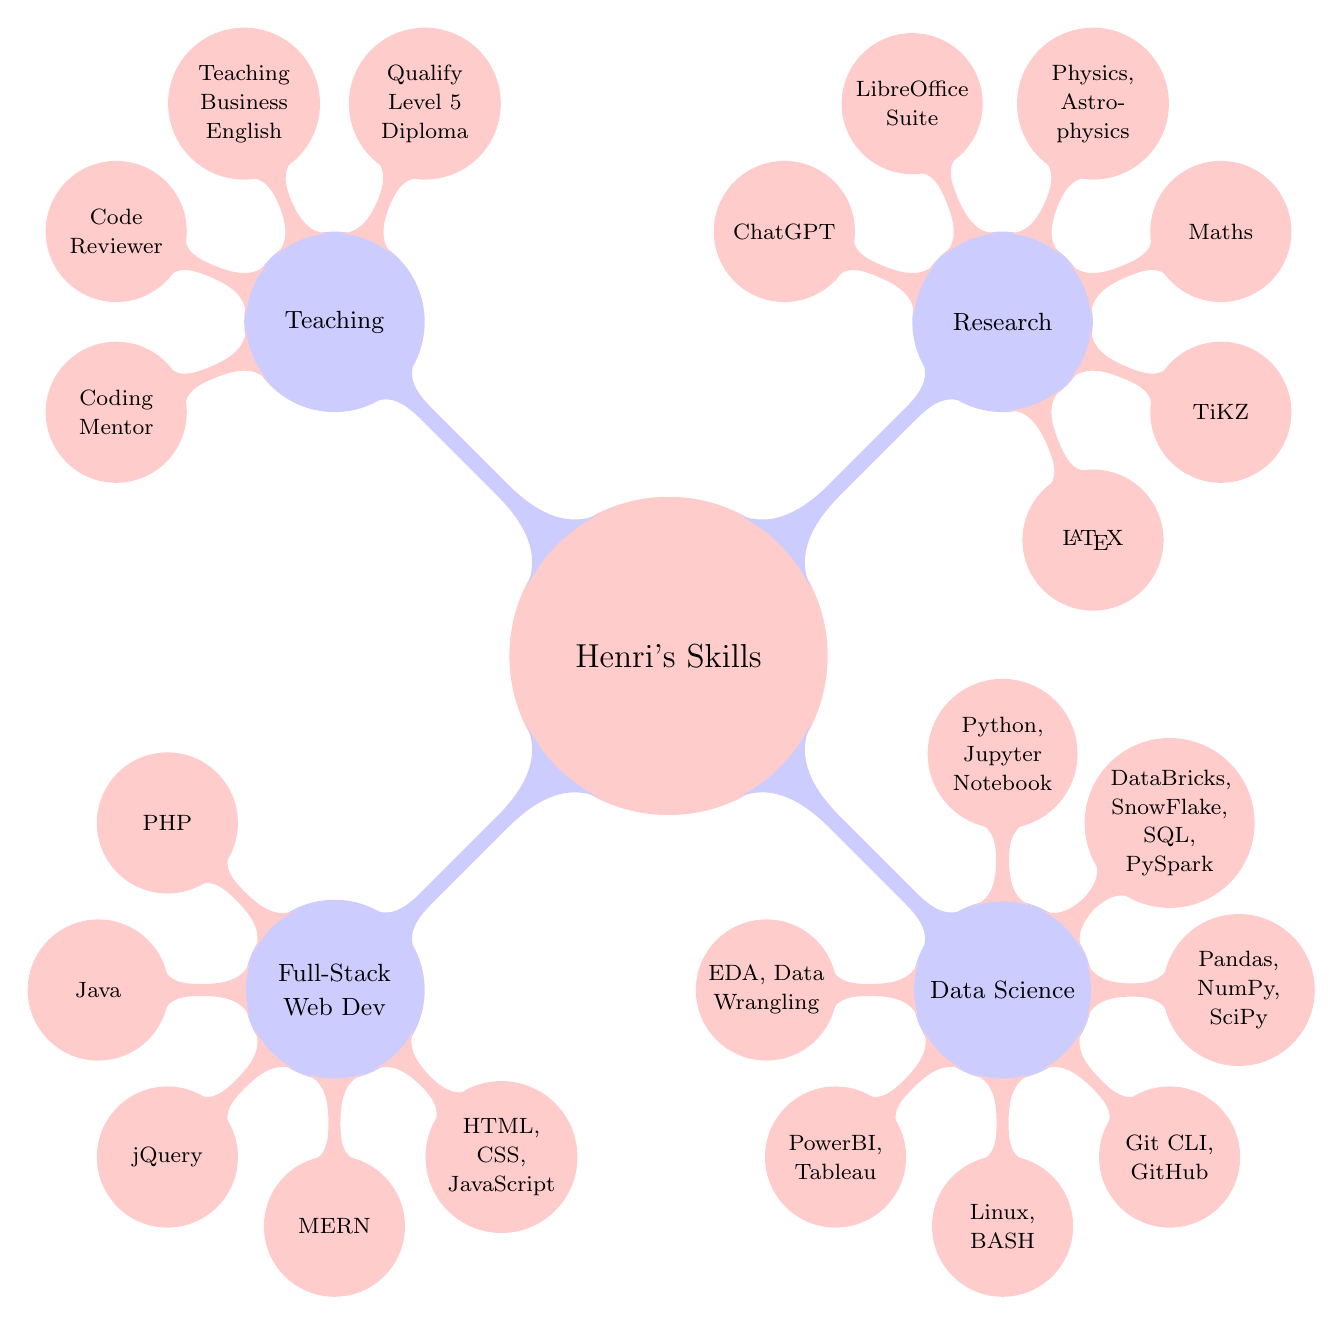
\begin{tikzpicture}
		\path[mindmap,grow cyclic, 
		every node/.style={concept, align=flush center},
		level 1/.append style={level distance=6cm, sibling angle=90, concept color=blue!20},
		level 2/.append style={level distance=3cm, sibling angle=45, concept color=red!20}]
		node[concept color=red!20]{Henri's Skills}
		child {node {Full-Stack \\ Web Dev}
			child {node {PHP}}
			child {node {Java}}
			child {node {jQuery}}
			child {node {MERN}}
			child {node {HTML, CSS, \\ JavaScript}}
		}
		child {node {Data Science}
			child {node {EDA, Data Wrangling}}
			child {node {PowerBI, Tableau}}
			child {node {Linux, BASH}}
			child {node {Git CLI, GitHub}}
			child {node {Pandas, NumPy, SciPy}}
			child {node {DataBricks, \\ SnowFlake, SQL, PySpark}}
			child {node {Python, \\ Jupyter Notebook}}
		}
		child  {node {Research}
			child {node {\LaTeX}}
			child {node {TiKZ}}
			child {node {Maths}}
			child {node {Physics, Astrophysics}}
			child {node {LibreOffice Suite}}
			child {node {ChatGPT}}
		}
		child  {node {Teaching}
			child {node {Qualify \\ Level 5 \\ Diploma}}
			child {node {Teaching \\ Business \\ English}}
			child {node {Code Reviewer}}
			child {node {Coding Mentor}}
		};	
	\end{tikzpicture}
\end{center}

\section*{References}
\begin{itemize}
	\item Seraaj De Villiers, HyperionDev, \href{mailto:seraajd@hyperiondev.com}{\textbf{seraajd@hyperiondev.com}}
	\item Prof. Christo Venter, North-West University, \href{mailto:christo.venter@nwu.ac.za}{\textbf{Christo.Venter@nwu.ac.za}}
	\item Mr. Jacobus Eksteen, CEO, Matogen Applied Insights, \href{mailto:jacobus.eksteen@ai.matogen.com}{\textbf{jacobus.eksteen@ai.matogen.com}}
\end{itemize}
	
\end{document}